\textit{Backpropagation} é um algorítmo de aprendizagem normalmente aplicado a MLP's que visa a aprendizagem baseada em correção de erros. Isso ocorre devido à retropropagação dos erros de saída de uma RNA pelas camadas anteriores, para que assim sejam balanceados os pesos de entrada da rede.
Este algorítmo possui três fases distintas:

\begin{itemize}
    \item Fase 1: Propagação dos sinais \\ Os sinais são propagados juntamente com os valores de entrada por todos os neurônios da rede a partir da entrada de dados até a camada de saída.
    \item Fase 2: Cálculo dos erros \\ Os erros são calculados nos neurônios de saída da rede para que sejam retropropagados.
    \item Fase 3: Retropropagação dos erros \\ Os erros que são encontrados nas camadas de saída, são propagados de volta para as camadas anteriores rebalanceando os pesos de entrada nas camadas superiores da rede. \cite{netto2006} Dessa forma a rede poderá chegar a resultados mais exatos nas próximas interações.
\end{itemize}

As duas fases descritas podem ser observadas na figura a seguir:

\begin{figure}[ht]
        \centering
        \label{fig05}
            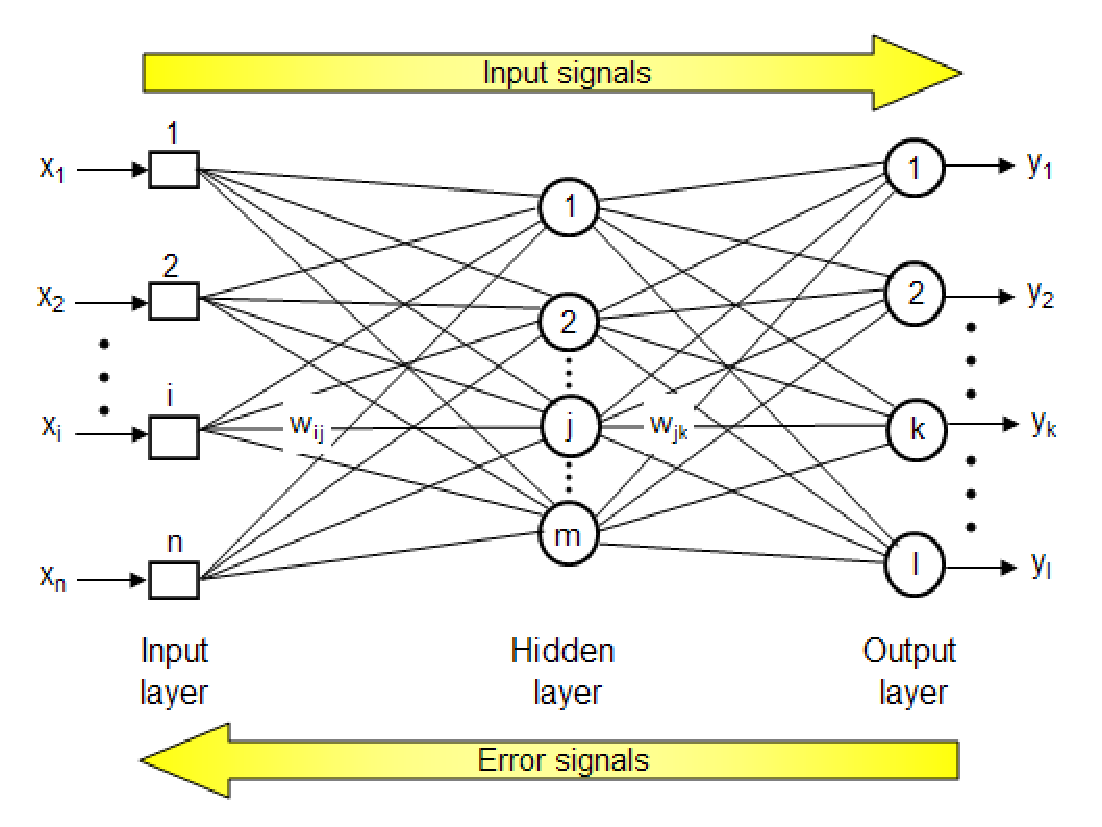
\includegraphics[keepaspectratio=true, scale=0.4]{editaveis/images/backprop.eps}
        \caption{Propagação de sinais de entrada e erros no \textit{Backpropagation}.}
        Fonte : \url{https://goo.gl/o7IGy4}
\end{figure}

